\section{Introducción}

La arquitectura propuesta se centra en la comunicación de la aviónica de un
vehículo espacial, con la característica de que sus componentes (nodos) son
de baja confiabilidad (se piensa en la utilización de compoentes COTS)
por lo tanto, es necesario que esta arquitectura sea tolerante a fallas. En este
trabajo el protocolo de comunicación (tolerante a fallas) propuesto,
se encuentra en las capas superiores del modelo de referencia OSI\footnote{ISO/IEC 7498-1 - Open System Interconnection}


Aquí hago la propuesta de la arquitectura.

El capítulo estará dividido en

\begin{itemize}
\item Arbol de requerimientos
\item Diseño estructural (Diagramas de bloques, bloques internos)
\item Diseño dinámico (Diagramas de secuencia, interacción, maquina de estados,)
  
\end{itemize}

\section{Árbol de requrimientos}
A continuación se detallas los requerimientos que van a guiar el diseño y
desarrollo de la propuesta de arquitectura de aviónica tolerantes a fallas
basada en componentes \ac{COTS} para satélites. En la Figura
\ref{fig:DiagramaRequerimientos} y en la Tabla \ref{table:Requerimientos} se pueden
observar los requerimientos. 

\begin{figure}[h!]
 \centering
 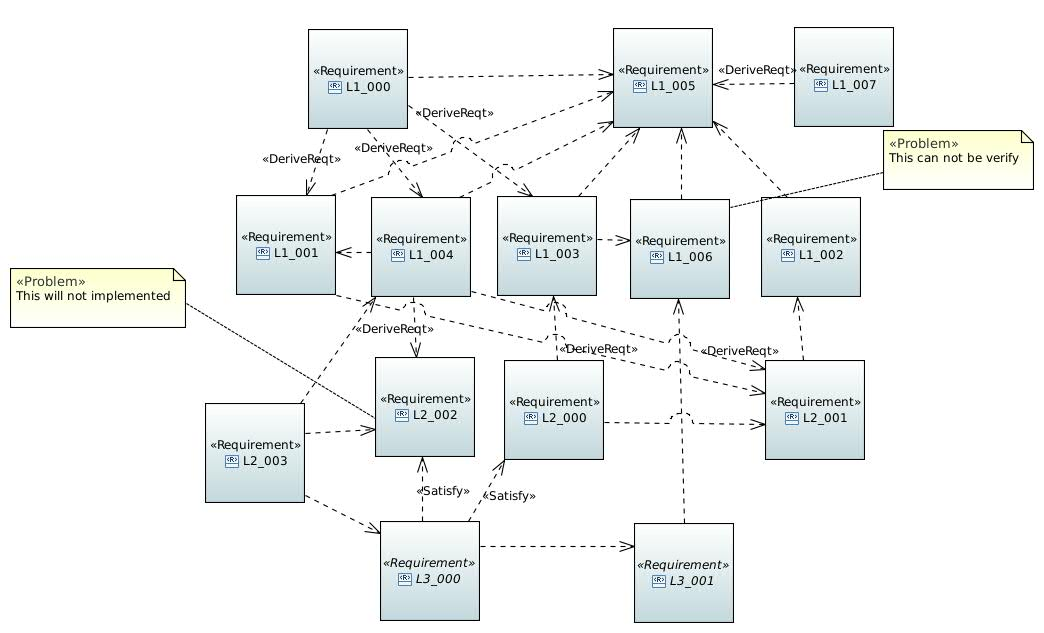
\includegraphics[scale=0.4]{images/Capitulo5/Diagrama_de_Requerimientos.JPG}
  \caption{Diagrama de requerimientos de la arquitectura propuesta}
\label{fig:DiagramaRequerimientos}
\end{figure} 

\begin{sidewaystable}[]
  \small
\centering
\caption{Tabla de requerimientos de la arquitectura propuesta}
\label{table:Requerimientos}
\begin{tabular}{|l|l|l|l|}
\hline
\multicolumn{1}{|c|}{\textbf{}} & \multicolumn{1}{c|}{\textbf{ID}} & \multicolumn{1}{c|}{\textbf{Name}} & \multicolumn{1}{c|}{\textbf{Detail}}                                                                           \\ \hline
0                               & L1\_001                          & L1\_001                            & The architecture components shall be Components Off-The-Shelf category                                         \\ \hline
1                               & L2\_000                          & L2\_000                            & The architecture shall be reconfigurate when a node fail.                                                      \\ \hline
2                               & L2\_001                          & L2\_001                            & Each subsystem shall represented for a Components Off-The-Shelf                                                \\ \hline
3                               & L1\_000                          & L1\_000                            & Shall be develop an avionics architecture for spacecraft using Components Off-The-Shelf                        \\ \hline
4                               & L1\_002                          & L1\_002                            & The architecture shall have at least 6 subsystems                                                              \\ \hline
5                               & L1\_003                          & L1\_003                            & The architecture shall have fault tolerance techniques to assurance the the mission life                       \\ \hline
6                               & L1\_004                          & L1\_004                            & The main bus to interconnect components shall be the Controller Area Network Bus developed for Bosch           \\ \hline
7                               & L1\_005                          & L1\_005                            & The architecture shall be sufficient to make a master degree thesis                                            \\ \hline
8                               & L2\_002                          & L2\_002                            & The architecture shall implements a based Controller Area Netoword protocol to intercommunicate the components \\ \hline
9                               & L3\_000                          & L3\_000                            & The intercommunication between nodes shall used the CANae protocol developed in the master degree thesis       \\ \hline
10                              & L1\_006                          & L1\_006                            & The architecture shall to assurance at least 10 years mission life                                             \\ \hline
11                              & L3\_001                          & L3\_001                            & The architecture shall use the distributed network philosophy                                                  \\ \hline
12                              & L1\_007                          & L1\_007                            & The thesis shall be finished in 1 year                                                                         \\ \hline
13 & L2\_003 & L2\_003 & The nodes shall send and receive message from any nodes connected to the architecture. \\ \hline
\end{tabular}
\end{sidewaystable}

A continuación se explica cada uno de los requerimientos:
\begin{itemize}
\item\textbf{L1\_000}: Este es el objetivo principal de la presente tesis:
  desarrollar una arquitectura de aviónica tolerante a fallas basada en
  componentes COTS para vehículos espaciales.
\item\textbf{L1\_001}: El principal requerimiento de este trabajo de tesis,
  es desarrollar una arquitectura basada en componentes COTS, lo cual agrega un
  grado importante de innovación tecnológica y complejidad, siendo de especial
  interés para INVAP trabajar con estos tipos de componentes.
\item\textbf{L1\_002}: Este requerimiento hace referencia que se debe asegurar
  el correcto funcionamiento de la arquitectura con una cantidad de al menos
  6 subsistemas.
\item\textbf{L1\_003}: Este requerimiento exige que la arquitectura sea
  tolerante a fallas para así poder sastifacer el requerimiento \textbf{L1\_006}.
\item\textbf{L1\_004}: Este requerimiento (constraint) indica que se debe pensar
  la arquitectura para ser utilizada con el bus CAN de Bosch. Este requerimiento
  es de interés par INVAP.
\item\textbf{L1\_005}: Este requerimiento indica que la arquitectura que se
  desarrolle debe ser sufiencite para lograr terminar una tesis de maestría. Por
  el diseño y desarrollo debe ser solo el suficiente y necesario para cumplir
  con el presente trabajo.
\item\textbf{L1\_006}: Este requerimiento indica que debe asegurarse que la
  arquitectura sea lo suficientemente robusta como para asegurar el el tiempo de
  vida de la misión de 10 años como mínimo. Existe un \textbf{problema} con este
  requerimiento, y es que para los alcances de esta tesis, será imposible
  verificar si se cumple con este requerimiento.
\item\textbf{L1\_007}: Este requerimiento indica que el trabajo de tesis tiene
  que ser finalizado en menos de un año. Esto tiene relación con el
  requerimiento \textbf{L1\_005} debido a que no se logrará alcanzar el detalle
  necesario para lograr la correcta implementación, verifación y validación de
  la arquitectura.
\item\textbf{L2\_000}: Este requerimiento exige que la arquitectura pueda
  reconfigurarse cuando un nodo falle.
\item\textbf{L2\_001}: Este requerimiento indica que para esta instancia de
  trabajo cada subsistema será tratado como un nodo dentro de la arquitectura.
\item\textbf{L2\_002}: Este requerimiento indica que se debe utilizar dentro de
  la arquitectura un protocolo de comunicación basado en el Bus CAN de Bosch.
\item\textbf{L2\_003}: Este requerimiento asegura que los nodos deben poder enviar
  y recibir mensajes de cualquier otro nodo conectado a la red CANae.
\item\textbf{L3\_000}: Este requerimiento indica que el protocolo de
  comunicación utilizado en esta arquitectura debe ser CANae. Este protocolo
  fue desarrollado en el presente trabajo de tesis (Vease:\ref{Appendix:A}).
\item\textbf{L3\_001}: Este requerimiento exige la utilización de una
  filosofía de red distribuída para su diseño y desarrollo.
\end{itemize}

\section{Casos de Uso}
A continuación se muestra el diagrama de Casos de Uso para la arquitectura propuesta.
El diagrama de Casos de Uso tiene como propósito explicar de manera general
el comportamiento a nivel de sistema de la arquitectura propuesta.
Los actores identificadores para esta arquitectura son los diferentes
subsistemas que se conectan a la red a través de los nodos.
Los subsistemas interactúan con el nodo a través de
la aplicación de usuario, es decir se encuentra asociados.
Se puede observar en la Figura \ref{fig:DiagramaCUArqPropuestaGENERAL}
que de forma general existen tres casos de usos que comprenden el comportamiento
general de la arquitectura. Se tiene \textit{Enviar mensaje} y \textit{Recibir
  Mensaje} los cuales son básicos para cualquier arquitectura de comunicación. A
esto se le agrega el caso de uso de \textit{FDIR} que es el agregado que se le
hace en este trabajo de tesis a través del protocolo de comunicación desarrollado
denominado CANae\ref{Appendix:A}. Debe aclararse que en 
la Figura \ref{fig:DiagramaCUArqPropuestaGENERAL}
aparece un resumen de los Actores intereactuando con el sistema. 

\begin{figure}[h!]
 \centering
 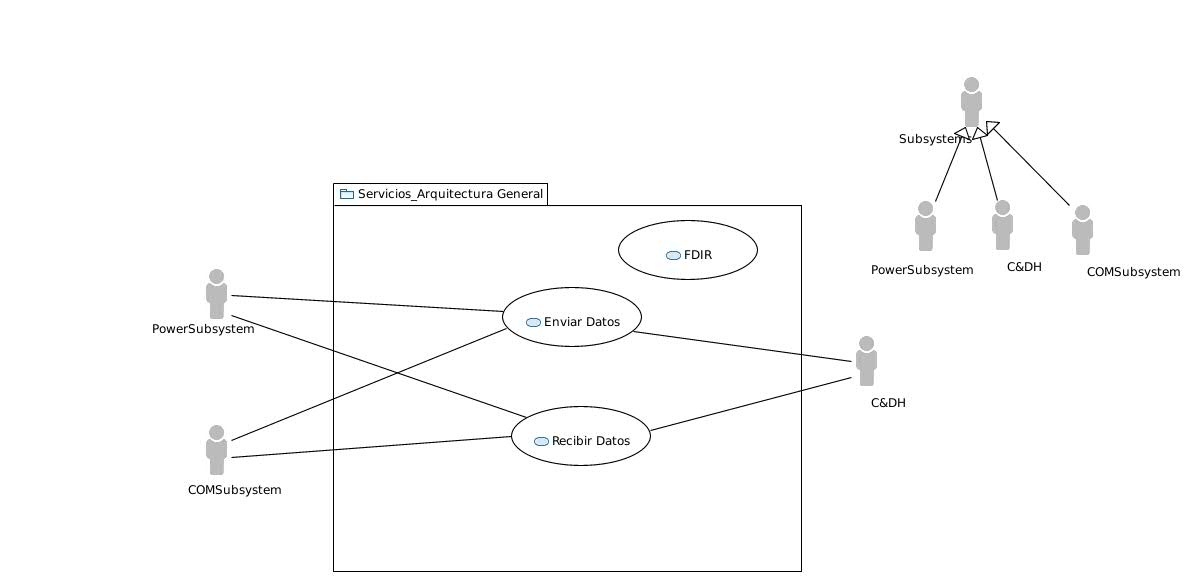
\includegraphics[scale=0.4]{images/Capitulo5/Arq_General.JPG}
  \caption{Diagrama de Casos de Uso General de la arquitectura Propuesta}
\label{fig:DiagramaCUArqPropuestaGENERAL}
\end{figure} 

De manera más detallada en la Figura \ref{fig:DiagramaCUArqPropuesta} se
observa un diagrama de casos de uso explayado. En este se pueden observar su
comportamiento.

\begin{figure}[h!]
 \centering
 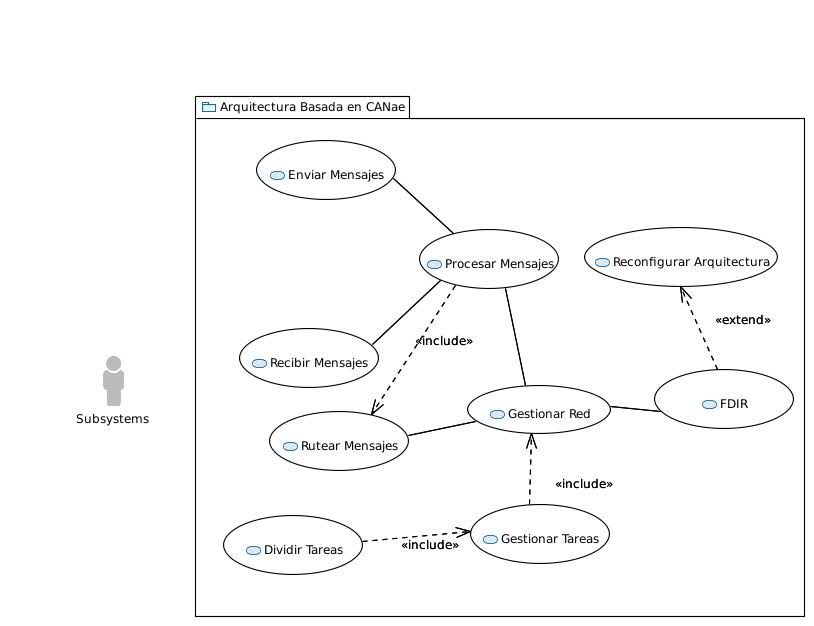
\includegraphics[scale=0.6]{images/Capitulo5/Caso_de_Uso_Arquitectura.JPG}
  \caption{Diagrama de Casos de Uso de arquitectura propuesta}
\label{fig:DiagramaCUArqPropuesta}
\end{figure} 

Le especifcación de los casos de usos se describen en \ref{Appendix:UseCase}.
Como se puede observar en la Figura \ref{fig:DiagramaCUArqPropuesta}
el sistema tiene 9 casos de uso.

Los casos de uso de \textit{Enviar Mensaje} y \textit{Recibir Mensaje} denota la
capacidad de la arquitectura de enviar y recibir mensajes (Data Frames de
CANae) desde y hacia las aplicaciones de usuario. Cuando una aplicación
necesita enviar un mensaje, estos deben primer pasar por el caso de uso
\textit{Procesar Mensaje} este es el encargado de empaquetar los mensajes.
También en este caso de uso se encuentra el caso de uso \textit{Rutear
  Mensaje}.

El caso de uso \textit{Rutear Mensaje} se encarga de aplicar los algoritmos
necesarios para lograr entregar el mensaje de una manera eficiente, siguiendo
la tabla de ruteo del CANae. Para esto se basa del caso de uso \texit{Gestionar
  Red}.

El caso de uso \texit{Gestionar Tareas} y \texit{Dividr Tareas} se encarga de
de conocer (periódicamente) el estado de la red y de sus nodos. Con esto puede
decidir cómo se reparten las tareas de una manera eficiente, siguiendo
la filosofía de arquitectura distribuída.

Por último tenemos el caso de uso \textit{FDIR} que hace referencia a la
Detección, Aislación, y Recuperación del sistema ante fallas. Debido a la
complejidad de esto, no se lo desarrolla a esta caso de uso en este trabajo.
El cual queda para \textbf{trabajos futuros}\ref{chap:TrabajosFuturos}. En este
caso de uso se encuentra el \textit{Reconfigurar Arquitectura}. Este es una
algoritmo del \ac{FDIR} que cuando se produce una falla en el algunos de los
nodos, la red se tiene que reconfigurar, para lograr continuar funcionando,
aún cuando haya nodos inactivos. Esto le brindaría a la arquitectura una grado
más de tolerancia a fallas. 

% talk about structural disegn
\section{Diseño Estructural}
gil

